%% DTK Domain Model

\documentclass[letterpaper,12pt]{article}
\usepackage[top=1.0in,bottom=1.0in,left=1.25in,right=1.25in]{geometry}
\usepackage{appendix}
\usepackage{verbatim}
\usepackage{amssymb}
\usepackage{graphicx}
\usepackage{longtable}
\usepackage{amsfonts}
\usepackage{amsmath}
\usepackage{algpseudocode} 
\usepackage[usenames]{color}
\usepackage[
  naturalnames = true, 
  colorlinks = true, 
  linkcolor = black,
  anchorcolor = black,
  citecolor = black,
  menucolor = black,
  urlcolor = blue
]{hyperref}
\usepackage{listings}
\usepackage{textcomp}

%%---------------------------------------------------------------------------%%
\author{
  Stuart R. Slattery\\
  Department of Engineering Physics\\
  University of Wisconsin - Madison\\
  1500 Engineering Dr.\\
  Madison, WI 53716\\
  \href{mailto:sslattery@wisc.edu}{\texttt{sslattery@wisc.edu}}
}

\date{\today}
\title{A Geometric Rendezvous-Based Domain Model for Data Transfer}
\begin{document}
\maketitle

\newpage

%%---------------------------------------------------------------------------%%
\begin{abstract}
  The Data Transfer Kit (DTK) is a software component designed to
  provide parallel services for mesh repartitioning, mesh searching,
  and data transfer for arbitrary physics components. In many physics
  applications, the concept of mesh is used to subdivide the physical
  domain into a discrete representation to facilitate the solution of
  the model problems that describe it. Additionally, the concept of
  the field is used to apply degrees of freedom to the mesh as an
  additional means of discretization. With the increased development
  efforts in multiphysics simulation, adaptive mesh simulations, and
  other multiple mesh problems, transferring fields and other data
  between meshes is a common operation. This document describes a
  domain model for mesh, fields, and parallel topology maps based on
  the concept of geometric rendezvous as developed in DTK.
\end{abstract}

\newpage

%%---------------------------------------------------------------------------%%
\section*{Acknowledgements}
This work was funded by the Consortium for the Advanced Simulation of
Light Water Reactors (CASL), a Department of Energy Innovation Hub
\cite{CASL_web}.

Thanks to Paul Wilson (University of Wisconsin), Greg Davidson and Tom
Evans (Oak Ridge National Laboratory), Roger Pawlowski (Sandia
National Laboratories) and the CASL team for their help and guidance
during the development of this work.

\newpage

%%---------------------------------------------------------------------------%%
\tableofcontents
\clearpage
\listoffigures
\clearpage
\newpage

%%---------------------------------------------------------------------------%%
\section{Introduction}\label{sec:intro}
In many physics applications, it is often desired to transfer fields
(i.e. degrees of freedom or other data) between meshes that may or may
not conform in physical space. In addition, for massively parallel
simulations, it is typical that meshes not only do not conform
spatially, but also that their parallel decompositions do not
correlate and are independent of one another due to physics-based
partitioning and discretization requirements. As an example, this
situation can occur in multiphysics simulations where physics fields
provide feedback between solution iterations or adaptive mesh
simulations where fields must be moved between meshes after refining
and coarsening. It is therefore desirable to have a set of tools to
relate two meshes of arbitrary parallel decomposition such that fields
and other data can be transferred between them.

The Data Transfer Kit (DTK) is a software component designed to
provide parallel services for mesh repartitioning, mesh searching, and
data transfer based on the concept of the rendezvous decomposition
\cite{Plimpton_2004}. To achieve a component design for use with
arbitrary physics codes, general concepts of mesh and fields are
employed to provide access to these services. This document will
outline the concepts of parallel communicators, mesh, fields, parallel
topology maps, and the rendezvous decomposition and how they are
modeled within the design of DTK.

\subsection{Basic Definitions}\label{subsec:basic_defs}

The following definitions are used throughout this document and serve
as a basis for the domain model and discussion.

\begin{itemize}
\item {\bf Communicator:} An object that allows communication of data
  between and controls the execution of operations on parallel
  processes.
\item {\bf Local Operation:} An operation that occurs within the
  context of a single process. All data and operations on that data
  are performed within the memory space of that process, independent
  of all other processes.
\item {\bf Global Operation:} An operation that occurs within the
  context of the entire parallel domain of the simulation. All data is
  potentially shared via communicator operations.
\item {\bf Ordinal:} A value that uniquely identifies an object from
  other objects of the same type. This number is positive and real
  such that for a given ordinal,$i$, $i \in \mathbb{R}^+$.
\item {\bf Geometry:} An object or collection of objects that has $n$
  physical dimensions and a spatial domain $\Omega \in \mathbb{R}^n$
  that is bounded by a boundary $\Gamma \in \mathbb{R}^n$.
\item {\bf Mesh:} An discrete representation of the $n$-dimensional
  spatial domain $\Omega \in \mathbb{R}^n$. Mesh can be considered a
  subset of geometry.
\item {\bf Field:} A discrete representaion of a $D$-dimensional
  function, $F$, over the domain $\Omega \in \mathbb{R}^n$ such that
  $F(r) : \mathbb{R}^n \rightarrow \mathbb{R}^D, \forall r \in
  \Omega$.
\item {\bf Evaluator:} An object that evaluates a field at a physical
  location, $\hat{r}$, in the spatial domain $\Omega$ by computing
  $F(\hat{r})$.
\item {\bf Source:} A geometry that owns a spatial domain, $\Omega_S
  \in \mathbb{R}^D$, over which an evaluator can be applied for a
  given field $F(s)$ where $s \in \Omega_s$.
\item {\bf Data Space:} A field, $G$, of dimension $D$, to which data
  can be applied such that $G(r) : \mathbb{R}^n \rightarrow
  \mathbb{R}^D, r \in \mathbb{R}^n$.
\item {\bf Target:} A geometry that owns a spatial domain, $\Omega_T
  \in \mathbb{R}^n$, over which a data space, $G(t)$ can be defined
  where $t \in \Omega_T$.
\item{ \bf Parallel Topology Map:} An operator, $M$, that defines the
  translation of a field, $F(s)$, from a source spatial domain,
  $\Omega_S$, to a field, $G(t$), in the target spatial domain
  $\Omega_T$, such that $M( F(r) ) : \mathbb{R}^D \rightarrow
  \mathbb{R}^D, \forall r \in \Omega_S \cap \Omega_T$, using both
  geometric and parallel operations.
\end{itemize}

\clearpage

%%---------------------------------------------------------------------------%%
\section{Communicators}\label{sec:communicators}
A communicator is a concept that encapsulates ownership of operations
in a parallel computation. A parallel communicator in the context of
DTK can be taken as a direct reference to a Message Passing Interface
(MPI) communicator \cite{MPI_1994}. A single communicator has a set of
process space over which it may perform operations. Multiple
communicators may exist in a single process space and own the same
processes. For objects decomposed in parallel, the term global will be
used to refer to concepts that apply across the entire parallel domain
owned by a communicator while the term local will be used to refer to
concepts that only exist in the domain of a single parallel process. A
communicator is not required to encompass all of global process
space. Based on this, we can consider union and intersection
operations.

\subsection{Communicator Union}\label{subsec:comm_union}
A union operation will compute the union in process space of all
communicators involved. This will be a common operation for cases
where one particular geometric component in the data transfer
operation is decomposed over a different communicator than another
geometric component. Figure~\ref{fig:comm_union} provides an example
of a union operation. In this example, two communicators, A and B, are
defined within the domain of a global communicator (typically, but not
necessarily MPI\_COMM\_WORLD) but do not encapsulate all of it. All
processes that exist either in communicator A or B will be used to
form the new union communicator ($C_{union}$) as a subset of the
global communicator ($C_{global}$) such that $C_{union} = A \cup B$
and $C_{union} \in C_{global}$. This operation is only valid if $A \in
C_{global}$ and $B \in C_{global}$.

\begin{figure}[htpb!]
  \centering 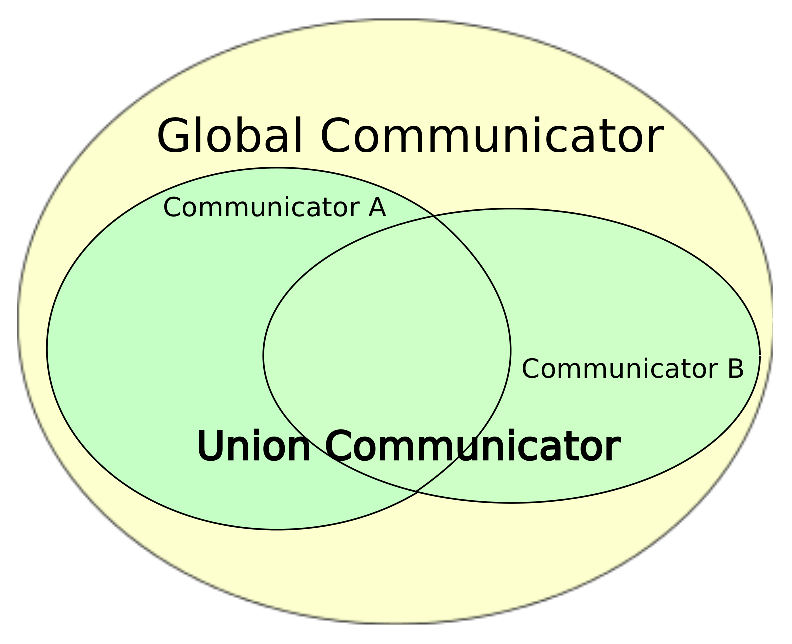
\includegraphics[width=5in]{union_comm.eps}
  \caption{\sl Communicator union operation diagram.}{\sl In this
    example, communicator A and communicator B are contained within
    the global communicator but do not encapsulate all of it. Their
    combined communication spaces form the union. The union is a
    subset of the global communicator.}
  \label{fig:comm_union}
\end{figure}

\subsection{Communicator Intersection}\label{subsec:comm_intersection}
An intersection operation will compute the intersection in process
space of all communicators
involved. Figure~\ref{fig:comm_intersection} provides an example of an
intersection operation. In this example, two communicators, A and B,
are defined within a global communicator but do not encapsulate all of
it. All processes that exist in both communicator A and B will be used
to form the intersection communicator. The intersection communicator
($C_{intersect}$) is a subset of the global communicator
($C_{global}$) such that $C_{intersect} = A \cap B$ and $C_{intersect}
\in C_{global}$. This operation is only valid if $A \in C_{global}$
and $B \in C_{global}$.

\begin{figure}[htpb!]
  \centering
  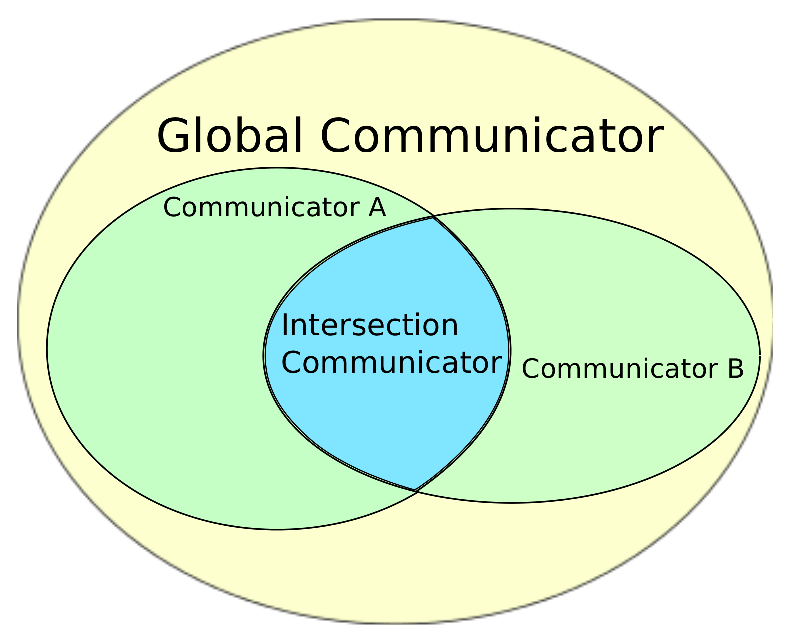
\includegraphics[width=5in]{intersection_comm.eps}
  \caption{\sl Communicator intersection operation diagram.}{\sl In
    this example, communicator A and communicator B are contained
    within the global communicator but do not encapsulate all of
    it. The blue communication space forms the intersection.}
  \label{fig:comm_intersection}
\end{figure}

\clearpage

%%---------------------------------------------------------------------------%%
\section{Mesh}\label{sec:mesh}
In order to access DTK mesh services, a subset of the information
needed to describe the mesh is required. This subset consists of nodes
and their coordinates, and elements and the nodes that construct
them. This subset has been demonstrated as sufficient for applying
data transfer algorithms \cite{Stewart_2004} and can be formulated in
such a way that algorithms can be generated that are data structure
netural \cite{Chand_2008}. In addition, for meshes that contain
multiple element topologies, the concept of mesh blocked by element
topology is utilized. 

\subsection{Mesh Nodes}\label{subsec:nodes}
Nodes are the lowest level geometric component of the mesh. All nodes
have a globally unique ordinal serving as an identification number for
the node in global operations. A node can have 1, 2, or 3 dimensions
but all nodes in a mesh must have the same dimension. To specify its
geometric position, each node has Cartesian (x,y,z) coordinates. A
node must provide only the coordinates for the specified node
dimension, no more or no less (e.g. a 2 dimensional node must provide
x and y coordinates but not a z coordinate). A node may be repeated
any number of times across the parallel domain with unlimited local
and global instances. However, every node with the same globally
unique ordinal must have the same coordinates. As an example, consider
Figure~\ref{fig:mesh_nodes} depicting a series of nodes contained in
a mesh. Each node provides a globally unique ordinal and set of 3
dimensional coordinates.

\begin{figure}[htpb!]
  \centering
  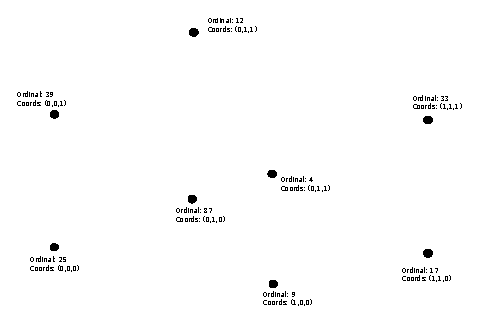
\includegraphics[width=5in]{hex_nodes.eps}
  \caption{\sl Basic node description for a mesh.}{\sl Each node is
    required to have a unique global ordinal, a specified
    dimensionality, and Cartesian coordinates corresponding to that
    dimensonality. The nodes in this example are 3 dimensional.}
  \label{fig:mesh_nodes}
\end{figure}

\subsection{Mesh Elements}\label{subsec:elements}
Elements are the second level of abstraction in the mesh description
above nodes. All elements have a globally unique ordinal serving as an
identification number for the element in global operations. This
globally unique ordinal can be the same as a globally unique ordinal
for a node in the mesh as DTK distinguishes between nodes and
elements. An element has a topology defining its physical structure
(e.g. tetrahedron, hexahedron, etc.) and a number of nodes needed to
generate that topology. Elements are constructed from nodes via a
connectivity list. The connectivity list for a particular element will
contain the unique node global ordinals that construct it. An element
may be repeated any number of times across the parallel domain
(i.e. it may have unlimited local instances), however, every globally
unique ordinal must have the same connectivity list associated with
it. For consistency, DTK uses the MoaB Canonical Numbering (MBCN)
scheme as a canonical ordering scheme \cite{Tautges_2009}. Each
element in a client mesh can be described with a connectivity list
using any canonical scheme of choice, however, the relationship
between this canonical numbering scheme and the DTK canonical
numbering scheme must be made available. Each element topology is
therefore also described by a permutation list. A permutation list
specifies the variation in ordering between the DTK canonical
numbering scheme and the client canonical numbering scheme. For
elements that have a higher order basis (e.g. quadratic), DTK resolves
these as higher order nodes via the MBCN system. See
Appendix~\ref{apdx:cell_topo} for canonical element topologies as
defined by DTK.

Consider the continuation of our example in
Figure~\ref{fig:mesh_element} showing a linear hexahedron element
generated from the nodes in Figure~\ref{fig:mesh_nodes}. The element
has been given a unique global ordinal and the connectivity and
permuation lists have been specified. The connectivity list specifies
an element construction from counter-clockwise movement around the
bottom face and then counter-clockwise movement around the top face
that is native to the client. The MBCN canonical ordering for linear
hexahedrons is given at the nodes. Note that MBCN ordering instead
uses clockwise rotation around the bottom and top faces to construct
the element. This difference in ordering is specified by the given
permutation list.

\begin{figure}[htpb!]
  \centering
  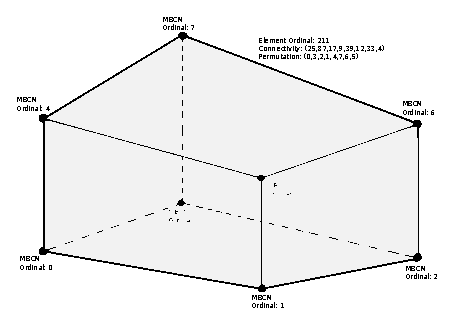
\includegraphics[width=5in]{hex_element.eps}
  \caption{\sl Basic element description for a mesh.}{\sl Each element
    is required to have a unique global ordinal, and a specified
    connectivity and permuation list. The MBCN canonical ordinals used
    by DTK are specified at the nodes.}
  \label{fig:mesh_element}
\end{figure}

\subsection{Mesh Blocks}\label{subsec:blocks}
At the highest level of abstraction, the mesh is composed of mesh
blocks. All elements in a block must have the same topology and number
of nodes. A mesh may contain as many blocks as desired. Multiple
blocks with the same mesh topology may exist. Nodes may be repeated in
different mesh blocks provided that they maintain the same unique
global ordinal and coordinates. Elements may be repeated in different
mesh blocks provided that they maintain the same unique global ordinal
and connectivity list. All elements and nodes in all blocks of the
mesh must have the same dimension. Multiple mesh blocks may exist in
the same spatial region as they are merely a means of subdividing the
mesh into groups of elements based on their topology. This behavior
will be the common when hybrid meshes are involved (e.g. a mesh that
contains hexahedrons and tetrahedrons). Mesh blocks may be either
structured or unstructured.

As an example, consider the 2 dimensional hybrid mesh presented in
Figure~\ref{fig:hybrid_mesh}. This mesh contains both quadrilateral
(blue) and triangle (red) elements that share connecting nodes. In
this case, all quadrilaterals should be specified in a single mesh
block and all triangles specified in another mesh block. The nodes
shared by these two mesh blocks may be repeated in either block.

\begin{figure}[htpb!]
  \centering
  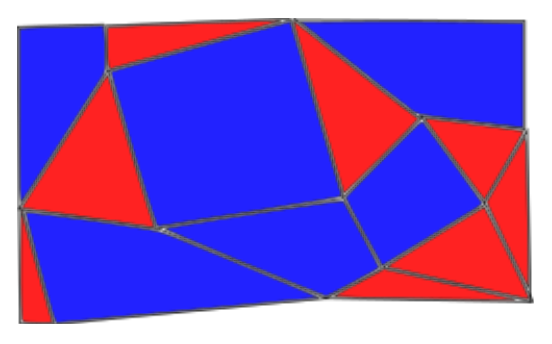
\includegraphics[width=5in]{hybrid_mesh.eps}
  \caption{\sl Hybrid mesh example.} {\sl Quadrilaterals (blue) must
    be specified in a different mesh block than the triangles
    (red). Both blocks can share the mutual mesh nodes that construct
    their elements.}
  \label{fig:hybrid_mesh}
\end{figure}

\subsection{Parallel Decomposition}\label{subsec:mesh_decomp}
Mesh blocks and the elements and nodes they contain may be partitioned
in any fashion provided that all nodes, elements, and blocks of a mesh
description exist in a communication space operated on by the same
parallel communicator. Different blocks in a single mesh description
may not have different communicators. Each mesh description may have
its own communicator. Global knowledge of the parallel decomposition
of a given mesh description is not required. Only local mesh data
access along with the proper communicator is required.

\clearpage

%%---------------------------------------------------------------------------%%
\section{Fields}\label{sec:field}
In the most general sense, a field refers to the degrees of freedom
computed by a physics code or the responses derived from those degrees
of freedom that have been discretized across the domain
\cite{LIME_2011}. In a physics simulation, examples of degrees of
freedom include pressure and velocity distributions and examples of
computed reponses include heat flux or reaction rates. In order to
access DTK field services, a subset of information needed to describe
the field is required. A field has a dimension of arbitrary size. As
examples, for scalar fields this dimension is 1, for 3-vectors (such
as the velocity example above in a 3 dimensional computation) is 3,
and for a 3x3 tensor the dimension is 9.  All local instances of the
field must have the same dimension. A field can have an arbitrary
number of local degrees of freedom and this size can differ from local
domain to local domain. No knowledge of the global field decomposition
is required, however, it must exist on a single communicator.


\subsection{Field Evaluations}\label{subsec:field_eval}
The actual discretization of the field is not explicitly
formulated. Rather, access to discretization of fields and the
associated data is generated through function evaluations at points in
physical space. Consider a $D$-dimensional function $F(r)$ of
arbitrary discretization over the spatial domain $\Omega \in
\mathbb{R}^n$ where $r \in \mathbb{R}^n$ and $F : \mathbb{R}^n
\rightarrow \mathbb{R}^D$. Via polynomial interpolation, projection,
or any other means necessary to most appropriately reflect the
discretization of $F(r)$, it then follows that evaluation operations
of the following type can be performed:

\begin{equation}
  \hat{f} \leftarrow F(\hat{r}), \forall \hat{r} \in \Omega
  \label{eq:evaluation}
\end{equation}

where $\hat{r} \in \mathbb{R}^n$ is a single point and $\hat{f} \in
\mathbb{R}^D$ is representative of the function $F(r)$ evaluated at
$\hat{r}$. This operation is not valid for $\hat{r} \notin \Omega$. In
the context of $\Omega$ discretized by a mesh, these evaluations can
instead be written in terms of a single mesh element, $\omega \in
\Omega$. 

\begin{equation}
  \hat{f} \leftarrow F(\hat{r}), \forall \hat{r} \in \omega
  \label{eq:element_evaluation}
\end{equation}

This operation is then not valid for $\hat{r} \notin \omega$. If
$\hat{r} \notin \omega$ and $\hat{r} \notin \Omega$, then alternative
schemes may be chosen, such as extrapolation, in order to apply the
field to $\hat{r}$.


\subsection{Basic Field Operations}\label{subsec:field_ops}
For various data transfer and error analysis routines, a suite of
common global operations on fields will be required. This includes
norm operations for a given field, $f$, of length $I$ and dimension
$D$ formulated for the $d^{th}$ dimension as the infinity norm:

\begin{equation}
  ||f_d||_\infty = \max_{1 \leq i \leq I} |{f_d}_i|
  \label{eq:infinity_norm}
\end{equation}

the 1-norm:

\begin{equation}
  ||f_d||_1 = \sum_{i=1}^I |{f_d}_i|
  \label{eq:one_norm}
\end{equation}

the 2-norm:

\begin{equation}
  ||f_d||_2 = \sqrt{ \sum_{i=1}^I |{f_d}_i|^2 }
  \label{eq:two_norm}
\end{equation}

and in general the q-norm:

\begin{equation}
||f_d||_q = \Bigg[ \sum_{i=1}^I |{f_d}_i|^q \Bigg]^{1/q}
  \label{eq:q_norm}
\end{equation}

all of which are valid over each dimension, $d$, of the field
\cite{LeVeque_2007}. In addition, other useful operations include a
global average over dimension:

\begin{equation}
  \bar{f_d} = \frac{1}{I}\sum_{i=1}^I {f_d}_i
  \label{eq:average}
\end{equation}

and scaling a field by a scalar multiple, $\alpha$.

\begin{equation}
  g_d = \alpha f_d
  \label{eq:field_scaling}
\end{equation}

where $\alpha \in \mathbb{R}$ and $g_d$ is the $d^{th}$ dimension of
the resulting scaled field.

\clearpage

%%---------------------------------------------------------------------------%%
\section{Geometric Rendezvous}\label{sec:rendezvous}
Relating two non-conformal meshes will ultimately require some type of
evaluation algorithm to apply the data from one geometry to another as
specified by Eq.~(\ref{eq:evaluation}). To achieve this, the target
objects to which this data will be applied must be located within the
the source geometry. In a serial formulation, efficient search
structures that offer logarithmic asymptotic time complexity are
available to perform this operation. However, in a parallel
formulation, if these two geometries are arbitrarily decomposed,
geometric alignment is not likely and a certain degree of
communication will be required. A geometric rendezvous manipulates the
source and target geometries such that all geometric operations have a
local formulation.

A geometry that is associated with the data that will be transferred
will be referred to as the source geometry while the the geometry that
will be receiving the data will be referred to as the target
geometry. Although explicitly formulated with a source mesh and target
nodes below, these concepts can be applied to geometric structures
beyond mesh and nodes.

\subsection{The Rendezvous Algorithm}\label{subsec:rendezvous_alg}
The geometric rendezvous concept uses a global formulation for the
data transfer while maintaining a local formulation for the geometric
search operations. In DTK, the following algorithm generated by
Plimpton et. al. \cite{Plimpton_2004} generates the rendezvous
decomposition through global operations in order to achieve a local
framework for geometric operations. 

\begin{enumerate}
\item Compute a box that bounds the source and target geometry
  intersection.
\item Create a rendezvous decomposition by performing recursive
  coordinate bisectioning on the source geometry.
\item Send source geometry from the source decomposition to rendezvous
  decomposition.
\item Clone source geometry components which overlap into nearby
  recursive coordinate bisectioning sub-domains.
\item Build a kD-tree with the local mesh in each rendezvous
  partition.
\end{enumerate}

This algorithm is elaborated in more detail in the following
paragraphs.

\paragraph{Step 1: Bounding box construction.}
To begin, a global bounding box for the source and target geometries
is constructed using their nodal data. These two bounding boxes are
then intersected to produce the bounding box around the intersection
of the two geometries. Those source or target nodes that are not
inside this intersection bounding box are not considered for the
remainder of the algorithm. This step is motivated by the fact that
for many classes of data transfer problems, such as 2 dimensional
surface transfer in a full 3 dimensional problem, only a small subset
of the source and target geometries will be used. This will reduce the
number of search operations and communication operations.

\paragraph{Step 2: Rendezvous decomposition generation.}
Recursive coordinate bisectioning (RCB) is used the create a new
decomposition with the source mesh nodes \cite{Berger_1987}.

\paragraph{Step 3: Send source elements to rendezvous decomposition.}
The RCB decomposition is generated only from source node
information. The element information must be sent to the rendezvous
decomposition for the point location process. 

\paragraph{Step 4: Clone source elements that overlap RCB
  sub-domains.}  Because RCB was performed using source nodal data,
there will be source elements that span the boundary between two or
more RCB sub-domains. When this occurs, the source elements will be
repeated in each RCB sub-domain in which their connectivity nodes
exist. 

\paragraph{Step 5: Build a kD-tree with the local mesh in each rendezvous
  partition.}  On each rendezvous process, the local mesh is be
searched with the local target nodes. A kD-tree is generated using the
local mesh for a fast proximity search of the domain that computes a
small subset of the local mesh that resides near the node
\cite{Bentley_1975}. This subset is then searched with a more
expensive point-in-element operation that transforms the node into the
reference frame of each element in the subset and uses a Newton
iteration strategy to determine if the node is contained within.

\subsection{The Rendezvous Decomposition}\label{subsec:rendezvous_decomp}
Using the above algorithm, a secondary decomposition of a subset of
the source mesh is generated forming the rendezvous decomposition. The
rendezvous decomposition is encapsulated as a separate entity from the
original geometric description of the domain. It can be viewed as a
copy of the source mesh subset that intersects the target
geometry. This copy has been repartitioned in a way that fundamental
geometric search operations are local and proceed globally in a load
balanced fashion.

The rendezvous decomposition has several properties. It is defined
over a communicator that encapsulates the union of the communication
spaces owned by the source and target geometries. It is defined inside
of a global, axis-aligned bounding box that bounds the intersection of
the source and target geometries. The decomposition is of the same
dimension as the source and target geometries. A rendezvous
decomposition cannot be generated with source and target geometries of
different dimensions (e.g. a 3 dimensional source geometry and a 2
dimensional target geometry cannot be used to generate a rendezvous
decomposition). 

Global recursive coordinate bisectioning parameters
are maintained for global partitioning information. A local kD-tree is
formed over the local mesh. In this way, mesh searches on the global
level use the RCB partitioning information and mesh searches on the
local level use the kD-tree.

\clearpage

%%---------------------------------------------------------------------------%%
\section{Parallel Topology Maps}\label{sec:map}

A parallel topology map is an operator, $M$, that defines the
translation of a field, $F(s)$, from a source spatial domain,
$\Omega_S$, to a field, $G(t$), in the target spatial domain
$\Omega_T$, such that $M( F(r) ) : \mathbb{R}^D \rightarrow
\mathbb{R}^D, \forall r \in [\Omega_S \cap \Omega_T$], using both
geometric and parallel operations. There are 3 types of parallel
topology maps: shared domain maps, interface maps, and network maps
\cite{LIME_2011}. Currently, DTK only supports shared domain maps,
however, interface and network maps are supported by this domain model
if the have a mesh-based formulation.

\subsection{Shared Domain Problems}\label{subsec:shared_domain}
A shared domain problem is one in which the geometric domains of the
source and target intersect over all dimensions of the
problem. Figure~\ref{fig:shared_domain} givens an example of a shared
domain problem in 3 dimensions. Here, $\Omega(S)$ (yellow) is the
source geometry, $\Omega(T)$ (blue) is the target geometry, and
$\Omega(R)$ (red) is their intersection and the shared domain over
which mapping and the rendezvous decomposition will be generated.

\begin{figure}[htpb!]
  \centering
  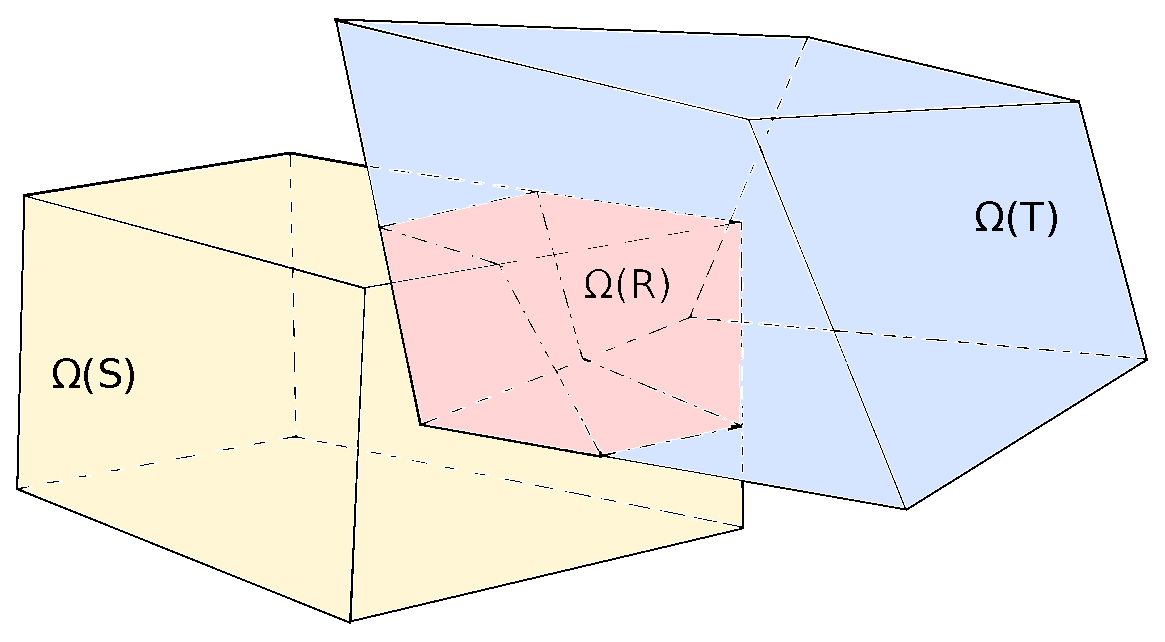
\includegraphics[width=5in]{overlapping_domain.eps}
  \caption{\sl Shared domain example.} {\sl $\Omega(S)$ (yellow)
    is the source geometry, $\Omega(T)$ (blue) is the target geometry,
    and $\Omega(R)$ (red) is the shared domain.}
  \label{fig:shared_domain}
\end{figure}

The shared domain map has several properties. It is defined over a
communicator that encapsulates the union of the communication spaces
owned by the source and target geometries.  The map is of the same
dimension as the source and target geometries. A shared domain map
cannot be generated with source and target geometries of different
dimensions (e.g. a 3 dimensional source geometry and a 2 dimensional
target geometry cannot be used to generate a shared domain map).

\subsubsection{Shared Domain Mapping Algorithm}
\label{subsubsec:shared_domain_alg}
The following mapping algorithm is applied using the rendezvous
decomposition to build a parallel topology map for share domain
problems.

\begin{enumerate}
\item Find which rendezvous sub-domain each target geometry component
  is inside of and determine the process which owns this sub-domain.
\item Send target geometry from target decomposition to rendezvous
  decomposition.
\item Find which target geometry component is inside which source
  geometry component.
\item Send source/target pairings from rendezvous decomposition to
  source decomposition.
\end{enumerate}

\paragraph{Step 1: Find rendezvous subdomain for target nodes.}
On each target process, the RCB decomposition is searched to find the
destination process for the target node in the rendezvous
decomposition.

\paragraph{Step 2: Send target nodes to rendezvous decomposition.}
Each target node is moved to the appropriate RCB sub-domain for the
point location step.

\paragraph{Step 3: Find the source elements in which target nodes reside.}
We now have source element information and target node information in
the rendezvous decomposition. On each rendezvous process, the local
mesh is searched with the local target nodes using the kD-tree and
underlying point-in-element functionality.

\paragraph{Step 4: Send element/node pairs back to original
  decompositions.}  The source element/target node pairs are the map
in this case and they will be used to drive the function evaluation
routines. These pairings must be communicated from the rendezvous
decomposition back to the source/target decompositions to complete the
mapping.


\clearpage

%%---------------------------------------------------------------------------%%
\bibliographystyle{ieeetr}
\bibliography{references}

\clearpage

%%---------------------------------------------------------------------------%%
\appendix
\section{DTK Element Topologies}\label{apdx:cell_topo}

\begin{figure}[htpb!]
  \centering
  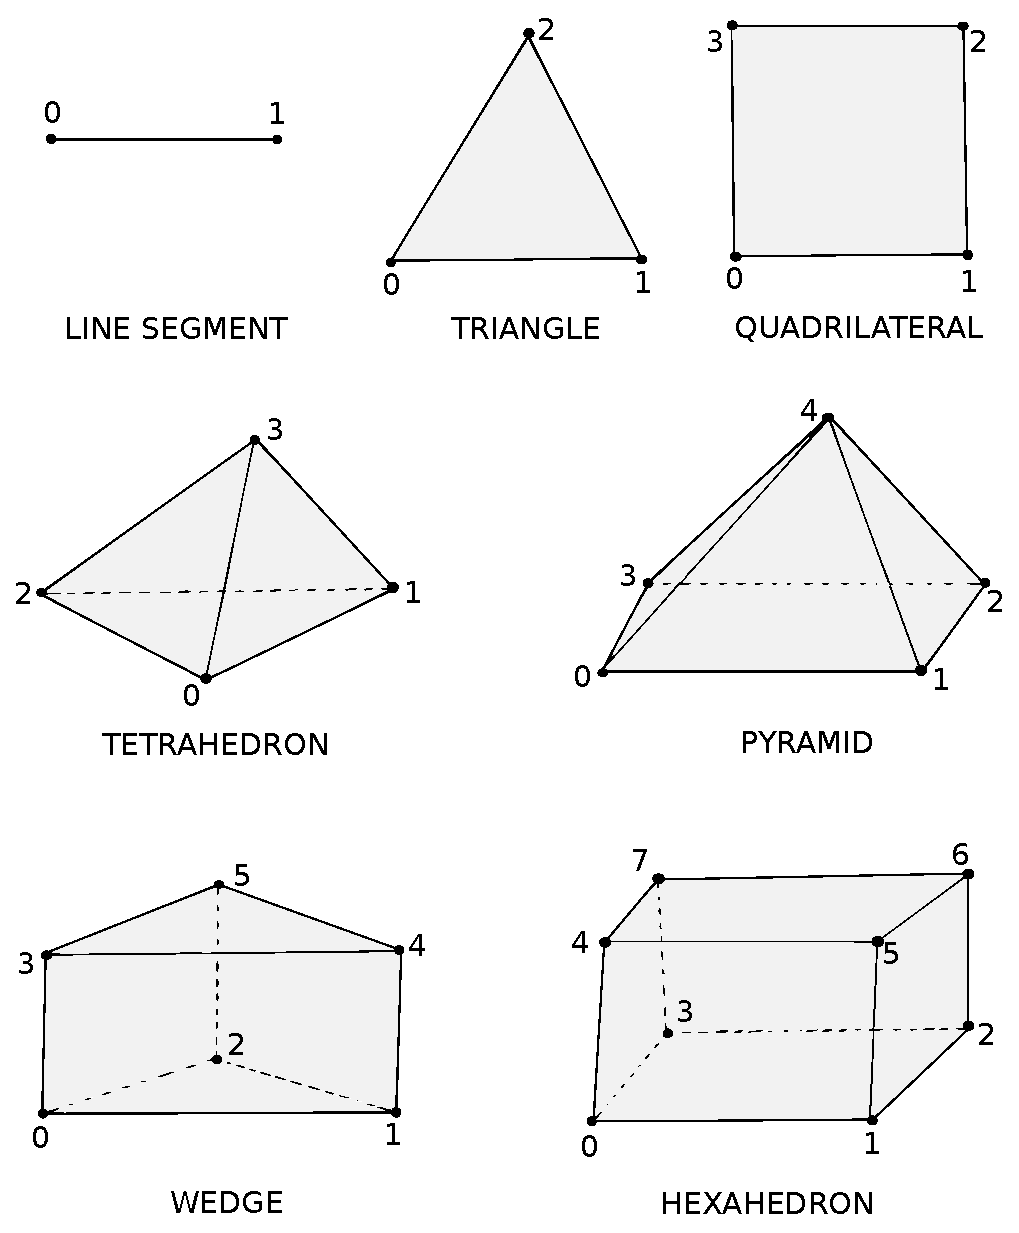
\includegraphics[width=5.5in]{Linear_Elements.eps}
  \caption{\sl Canonical connectivity schemes for linear elements in
    DTK}{\sl (a) line segment, (b) triangle, (c) quadrilateral, (d)
    tetrahedron, (e) hexahedron, (f) pyramid.}
  \label{fig:linear_elements}
\end{figure}

\clearpage

%%---------------------------------------------------------------------------%%
\end{document}


